\chapter{Ableitung der Schmerz Score}

In Kapitel \ref{sec:marking_cry-units_new} wurden Methoden vorgestellt, durch die einem Audiosignal die Cry-Units erkannt und markiert werden. Diese Cry-Units bilden den Ausgangspunkt, um eine Schmerz Score ableiten zu können. 

Wie in Kapitel \ref{sec:painScores} erläutert wurde, wird eine Schmerz Score typischerweise nicht aus den Informationen einer einzelnen Cry-Unit, sondern aus Gruppen mehrerer Cry-Units innerhalb eines längeren Beobachtungszeitraumes geschlossen. Dafür ist es zunächst notwendig, diejenigen Cry-Units zu identifizieren, die gemeinsam einem schmerzversuchanden Stimulus zugeordnet werden können. Diese Gruppierung von Cry-Units wird in dieser Arbeit als \emph{Segmentierung} bezeichnet und in Kapitel \ref{sec:segmenting} vorgestellt. Die so entstandenen Segmente bilden die Basis zur Ableitung von Schmerz Scores, welche in Kapitel \ref{sec:marking_cry-units_new} diskutiert wird.


\section{Segmentierung}
\label{sec:segmenting}


Wie in Kapitel \ref{sec:painScores} erläutert wurde, wird die Schmerzdiagnose für Post-Operativen Schmerz mit Pain Scales typischerweise umgesetzt, indem das Baby in bestimmten Intervallen besucht und für einen festgelegten Zeitraum beobachtet wird, worauf den Schmerzgrad für einen bestimmten Zeitpunkt diagnostiziert wird. So empfiehlt die Pain Scale PAT, das Baby alle 30 Minuten zu besuchen und für 15 bis 30 Sekunden zu beobachten. Für viele Pain Scales konnten diese  Beobachtungsintervalle und Zeiträume nicht in Erfahrung gebracht werden. 

Dieses Vorgehen der Schmerzdiagnose nur zu festgelegten Zeitintervallen macht keinen Sinn für ein kontinuierliches System, da es den Vorteil der Kontinuierlichkeit eliminieren würde. Die Frage ist also, wann eine medizinische Fachkraft den Anfangszeitpunkt einer Schmerzdiagnose festlegen würde, würde es das entsprechende Baby rund um die Uhr beobachten, und nicht nur eine Visite zu festgelegten Zeitpunkten durchführen. Die logisch nächstliegende Antwort ist, die Schmerzdiagnose genau dann zu starten, wenn das Baby anfängt, zu schreien. 

Die nächste Frage ist, wann man die Beobachtung wieder beendet und eine Schmerz Score für den beobachteten Zeitraum festlegt. Da einige Pain Scales aus Tabelle \ref{tab:painscores} Beobachtungszeiträume angeben, kann argumentiert werden, dass die Beobachtung direkt nach dem für die jeweilige Scale angegebenen Zeitraum beendet werden und eine Pain Score abgeleitet werden kann, auch, wenn das Baby weiterhin schreit. Dabei stellt sich die Frage, welche Zeiträume man für die Pain Scales festlegt, die keinen selber keinen vorschreiben. Die zweite Frage ist, ob eine Vorzeitige Beendigung der Beobachtung überhaupt sinnvoll ist, wenn ein automatisierte System zur Verfügung steht und der Beobachter somit \glqq unendlich viel Zeit hat\grqq . Daher wird an dieser Stelle zuerst die grundlegendere Frage gestellt: Was ist der längste sinnvolle Zeitraum, für den eine Pain Score abgeleitet werden kann? Die nächstliegende Antwort ist: Dann, wenn das Kind aufhört, zu schreien.

Auf Basis dieser Argumentation wurde das folgende Vorgehen zur kontinuierlichen Segmentierung entwickelt: Wenn das Baby keine Äußerungen von sich gibt, weil es beispielsweise schläft, wird keine Cry-Unit festgestellt, und somit existiert auch momentan kein offenes Segment. Fängt das Baby an, einen Laut von sich zu geben, also eine Cry-Unit zu produzieren, wird ein neues Segment eröffnet und die Cry-Unit diesem Segment hinzugefügt. Weitere Cry-Units werden so lange diesem Segment hinzugefügt, wie die Dauer der Stille nach einer Cry-Unit einen festgelegten Grenzwert $t_{s}$ nicht überschreitet. Ein Cry-Segment wird dann geschlossen, wenn das Baby für einen festgelegten Zeitraum keine Laute mehr von sich gibt, also \glqq aufhört, zu weinen\grqq{}. Das Endzeitpunkt des Segmentes wird als der Endzeitpunkt der letzten Cry-Unit des Segmentes festgelegt.

Formel \ref{eq:cry-segment}  definiert ein \emph{Cry-Segment} [$CS$] als Datentyp. Ein Cry-Segment ist eine Liste von Cry-Units. Alle Cry-Units erfüllen die Nebenbedingung \ref{eq:cry-segment-nb}, das heißt, dass die Distanzen aller benachbarter Cry-Units eines Cry-Segments unterhalb des Grenzwertes $t_{s}$ liegen.

\begin{equation}
CS = [cu_0 ,  \ldots,  cu_n]
\label{eq:cry-segment}
\end{equation}

\begin{equation}
\forall cs \in CS: \forall i = 0 \ldots length(cs)-2 : d(cs[i], cs[i+1]) < t_{s}
\label{eq:cry-segment-nb}
\end{equation}

Der Start-Zeitpunkt eines Cry-Segments wird nach Formel \ref{eq:cry-segment-start} als der Startzeitpunkt der ersten Cry-Unit des Segments definiert. Das Ende eines Segmentes wird definiert als der Endzeitpunkt der letzten Cry-Unit nach Gleichung \ref{eq:cry-segment-end}.

\begin{equation}
start(cs) = cs[0].start
\label{eq:cry-segment-start}
\end{equation}

\begin{equation}
end(cs) = cs[n].end
\label{eq:cry-segment-end}
\end{equation}

Algorithmus \ref{alg:crySegment} zeigt einen Pseudocode, wie die Segmentierung nach dem beschriebenen Prinzipien offline durchgeführt wird. Input des Algorithmus ist die Liste aller Cry-Units $CU_{all} = [cu_0 ,\ldots, cu_m]$, die durch das Decision-Smoothing nach Algorithmus \ref{alg:decisionSmoothing} entstanden ist. Das Ergebnis des Algorithmus ist die Liste $CS_{all}$, die alle gefundene Cry-Segmente  $[cs_0 , \ldots ,  cs_n]$ enthält. Der Algorithmus eignet sich nicht für eine Online-Segmentierung, da das Ende eines Segmentes erst bei Beginn eines neuen Segmentes festgestellt wird, wobei beliebig viel Zeit zwischen den Beiden Segmenten liegen kann. Wurde beispielsweise $t_{s} = \SI{1}{\minute}$ festgelegt, und die Pause zwischen zwei Segmenten beträgt eine Stunden, so wäre das Ende des ersten Segmentes 59 Minuten zu spät festgestellt worden. Bei einer online durchgeführten Segmentierung empfiehlt es sich, die Dauer der Stelle nach jeder neu erkannten Cry-Unit kontinuierlich zu Messen und ein Segment sofort zu beenden, wenn ein Stillezeitraum den Grenzwert $t_s$ überschreitet.

\begin{algorithm}[H]
	\caption{Gruppierung von Cry-Units zu Cry-Segments}
	\label{alg:crySegment}
	\begin{algorithmic}[1]
		\Function{segmentCryUnits}{$CU_{all}, t_{s}$}
		\State $ CS_{all} \gets [\;]$
		\State $ cs \gets [CU_{all}[0]]$
				\For{ $i = 1 , \ldots , length(CU_{all}) - 1$}
						\State $ cu_i \gets CU_{all}[i]$
						\State $cu_{i-1} \gets CU_{all}[i-1]$
						\If{d$(cu_{i-1},cu_i) < t_{seg-max}$}
								\State $cs \gets [cs_i , cu_i]$
						\Else
								\State $CS_{all} \gets [CS_{all}, cs]$
								\State $cs \gets [cu_i]$
						\EndIf
				\EndFor
		\Return $CS_{all}$
		
		\EndFunction
		
	\end{algorithmic}
\end{algorithm}

Abbildung \ref{img:segmenting06} zeigt die nach dieser Methode durchgeführte Segmentierung anhand eines Beispiels.

\begin{figure}[h]
	\centering
	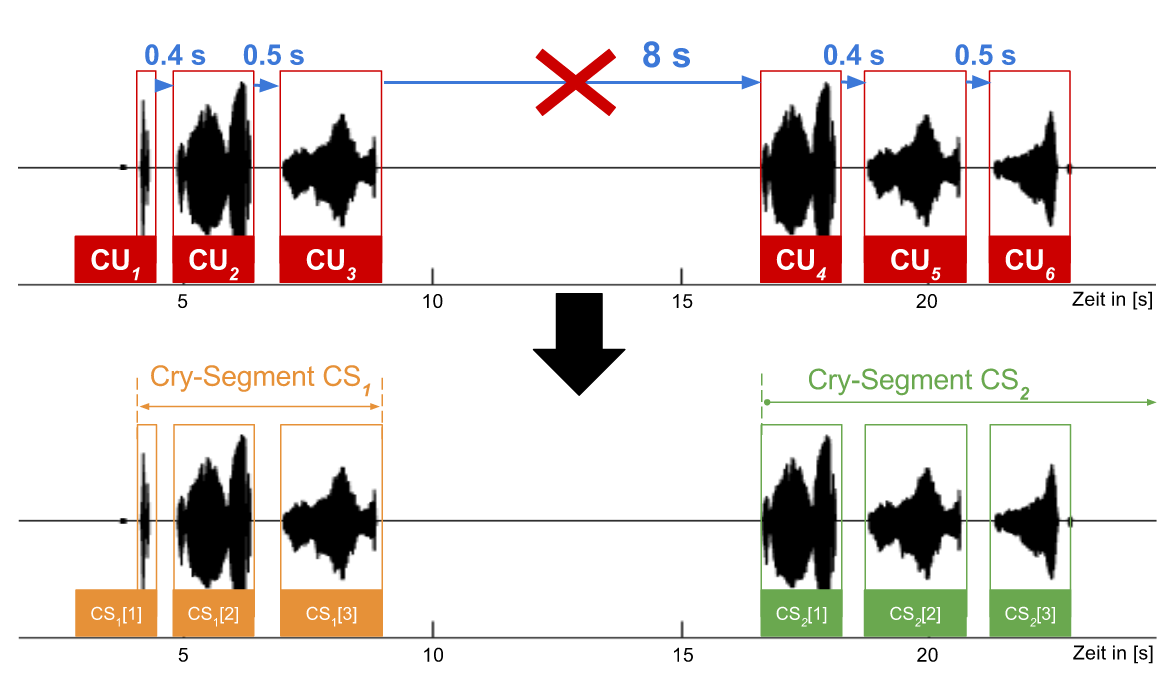
\includegraphics[width=1\textwidth]{bilder/segmentierung06.png}
	\caption{Beispiel für eine Segmentierung mit einem Grenzwert von $t_s = \SI{6}{\second}$}
	\label{img:segmenting06}
\end{figure}

Das hier vorgestellte Vorgehen wurde absichtlich möglichst einfach gehalten, damit der Sinn des Parameters $t_{s}$ leicht ersichtlich ist und somit von der medizinischen Fachkraft selbständig festgelegt werden kann. Schlussendlich ist eines der Hauptziele dieser Segmentierung, unnötige Berechnungen von Schmerz-Scores in den nachfolgenden Schritten zu vermeiden, so lange keine Cry-Units vorliegen. Das Ende eines Segmentes ist außerdem ein günstiger Zeitpunkt, um die Parameter des Kompressors im Pre-Processing auf Basis des RMS-Wertes des Segmentes zu aktualisieren (siehe Kapitel \ref{sec:preprocessing}). Trotz der Trivialität dieser laufenden Segmentierung liegt hier ein wichtiger Unterschied im Gegensatz zu vergleichbaren Systemen, wie zum Beispiel das von Cohen et al. \cite{cohenCry}, bei dem die Entscheidung über Cry/not-Cry für Segmente mit einer festen Fenstergröße von 10 Sekunden vorgenommen wird. 

\section{Extrahierung von Eigenschaften und Ableitung der Schmerzscore}
\label{sec:overviewPainRegression}

Das Ergebnis der Segmentierung ist eine Liste an Cry-Segmenten $cs_0,  \ldots , c_n$. Diese Cry-Segmente bilden nun die Basis für die Ableitung der Pain Score. Die medizinische Fachkraft, die das System verwendet, muss dabei zuerst die Wahl treffen, welche Pain Scale verwendet werden soll. Das einfachste denkbare Vorgehen ist die Ableitung genau einer Pain Score aus den globalen Eigenschaften eines Segmentes, wobei diese Ableitung erst vollzogen werden kann, sobald ein Segment abgeschlossen wurde und alle Informationen für dieses Segment vorliegen. Es wird also jedem Segment genau eine Pain Score zugewiesen. Das Vorgehen wird am Beispiel der NIPS aus Tabelle \ref{tab:nips} verdeutlicht: Dabei steht die Abwesenheit von Weinen für null Punkte, \glqq mumbling\grqq{} (murmeln) für einen Punkt und \glqq vigorous\grqq{} (energisch) für zwei Punkte. Bei Abwesenheit von Lautäußerungen, also der Zeitraum zwischen den Segmenten, werden also keine Punkte = null Punkte vergeben. Ein Segment, dessen Qualität insgesamt als \glqq murmelnd\grqq{} bewertet wird, erhält einen Punkt, und ein Segment, welches als insgesamt als \glqq energisch\grqq{} bewertet wird, zwei Punkte. Das Problem ist offensichtlich: \glqq murmelnd\grqq{} und \glqq energisch\grqq{} sind subjektiv behaftete Begriffe und lassen sich nicht ohne weiteres aus den Eigenschaften eines Segmentes feststellen. 

Es werden zwei verschiedene Lösungs-Strategien für dieses Problem vorgestellt. 

\vspace{5mm}

\textbf{Strategie 1} \noindent\rule{0.83\linewidth}{0.3pt}\\
... löst das Problem mit Hilfe von \emph{Regression} (Siehe Kapitel \ref{sec:regression}):
\begin{enumerate}
 \item Man erstellt eine Datenbank mit Aufnahmen von kindlichen Lautäußerungen, die man segmentiert.
 \item Man errechnet \glqq so viele \emph{objektiv} messabare Eigenschaften wie möglich\grqq{} für jedes Segment, wie zum Beispiel die insgesamte Länge, die durchschnittliche Länge der enthaltenen Cry-Units, durchschnittliche Tonhöhe usw.
 \item Man bittet medizinische Fachkräfte, für jedes Segment der Datenbank eine Score bezüglich einer Pain Scale zu vergeben. Dadurch erhält man eine gelabelte Test-Datenbank.
 \item Man verwendet einen \emph{Regressionsalgorithmus}, um den Zusammenhang zwischen den in Schritt 2 objektiv gemessenen Eigenschaften der Segmente und den in Schritt 3 vergebenen \emph{Scores} herzustellen. An dieser Stelle kann zum Beispiel die in Kapitel \ref{sec:multipleRegression} beschriebene multiple lineare Regression verwendet werden. Man erhält somit einen Regressor für jede Pain Scale.
 \item Möchte man für neue, unbekannte Segmente die Pain Score prognostizieren, nutzt man den entsprechenden Regressor.
\end{enumerate}
\noindent\rule{\linewidth}{0.3pt}

Das Vorteil dieses Vorgehens ist, dass das Problem der Übersetzung der objektiv messbaren Parameter in die subjektiv behafteten Begriffe überbrückt wird, indem die Regression direkt von den objektiv messbaren Parametern auf  die Pain Score durchgeführt wird. Der Nachteil ist, dass eine Testdatenbank für jede Pain Scale aufgebaut werden muss. Wird ein neue Pain Scale eingeführt, muss der Regressor für diese Scale durch erneutes Labeln festgestellt werden. Ein weiterer Effekt der Abbildung des Problems als Regression ist, dass ein Regressor in einen kontinuierlichen Zahlenraum abbildet. Es sind also Regressionsergebnisse wie zum Beispiel $2.8$ denkbar. Diese \glqq bessere Auflösung\grqq{} kann als Vorteil betrachtet werden. Ist jedoch eine direkte Übersetzung der Pain Scale inklusive der ganzzahligen Punktzahlen gewünscht, so stellt sich die Frage, ob eine $2.8$ auf- oder abzurunden ist.

\vspace{5mm}

\textbf{Strategie 2} \noindent\rule{0.83\linewidth}{0.3pt} \\
... löst das Problem mit Hilfe von Klassifizierung (Siehe Kapitel \ref{sec:classification}):
\begin{enumerate}
	\item und 2. entsprechen Strategie 1
	\stepcounter{enumi}
	\item Man sammelt alle subjektiven Begriffe, die in Pain Scales verwendet werden, wie zum Beispiel \glqq murmelnd\grqq , \glqq energisch\grqq , usw.
	\item Man bittet medizinische Fachkräfte, jedes Segment der Datenbank mit denjenigen Begriffen zu labeln, die die jeweilige Person für zutreffend hält. 
	\item  Man Verwendet einen \emph{Klassifizierungsgorithmus}, um einen Zusammenhang zwischen den in Schritt 2 festgestellten objektiv messbaren Eigenschaften der Segmente und den \emph{subjektiv behafteten Begriffen} zu finden. Man erhält somit einen Klassifikator für jeden Begriff, der binär in \emph{positive = zutreffend} und \emph{negative = nicht zutreffend} klassifiziert.
	\item Möchte man für neue, unbekannte Segmente die Pain Score prognostizieren, so wird für jede mögliche Score der Pain Scale überprüft, ob für alle subjektiv beschreibenden Begriffe der entsprechende Klassifikator ein positive prognostiziert. Die Ableitung der Score ist somit ein weiters Klassifizierungsproblem, wobei eine Score einer Klasse entspricht und genau dann abgeleitet werden kann, wenn alle Vorraussetzungen für die Klasse erfüllt sind.
\end{enumerate}
\noindent\rule{\linewidth}{0.3pt}

Der Vorteil dieser Methode ist, dass auch zum Zeitpunkt der Erstellung der Testdatenbank unbekannte Pain Scales zu einem späteren Zeitpunkt eingebunden werden können, insofern alle in dieser neuen Pain Scale verwendeten subjektiv behafteten Begriffe bereits gelabelt vorliegen, weil sie auch in anderen Pain Scales verwendet wurden. Das Vorgehen erlaubt somit eine gewissen Flexibilität bezüglich zukünftig entwickelter Pain Scales. Der Nachteil dieser Methode ist, dass durch die Umwandlung der eigentlich quantitativ geordenten Score einer Pain Scale in qualitative Klassen aus einem implizit als Regression zu betrachtenden Problem ein Klassifizierungsproblem macht. Dies wirft neue Fragen auf, wie zum Beispiel: Angenommen, bei einer fiktiven Pain Scale wird jede Score mit jeweils drei subjektiv behafteten Begriffen beschrieben, und bei der Klassifizierung eines Segmentes wird festgestellt, dass für jede Punktzahl genau zwei der drei Begriffe erfüllt werden. Welche Score wird dann prognostiziert? Ein anderes Beispiel wird am Beispiel der der NIPS-Score aus Tabelle \ref{tab:nips} verdeutlicht: Angenommen, ein Cry-Segment enthält hörbar \glqq starkes\grqq{} Schreien, es kann jedoch weder \glqq mumbling (murmelnd) \grqq{} noch \glqq vigorous (energisch)\grqq{} abgeleitet werden. Demzufolgen müsste dieses Segment eine Score von 0 Punkten erhalten, wobei ein Mensch in dieser Situation eventuell \glqq stark\grqq{} zu \glqq heftig\grqq{} uminterpretieren und 2 Punkte vergeben hätte. Strategie 1 ist weniger anfällig für dieses Problem.

In jedem Fall werden medizinische Fachkräfte benötigt, um das Labeling der Cry-Segmente durchzuführen, was aus Zeitgründen im Rahmen dieser Arbeit nicht möglich ist. Die Aquise von Audioaufnahmen von Babys sowie das Labeling der Aufanhmen erfodern nicht nur Zeit, sondern das Fachwissen über das Führen und die Auswerten von Interviews.

\subsection{Extrahierung von Eigenschaften}
\label{sec:segmentFeatures}

Im vergangenen Kapitel wurde erläutert, dass die Basis für die Ableitung einer Pain Score für ein Segment die Extraktion von \glqq so vielen Features wie möglich\grqq{} ist. In diesem Kapitel wird präzisiert, welche Features gemeint sind.  Varallyay \cite[S. 16 - 17]{cry_thesis} schlug vor, drei Kategorien an Features zu betrachten: 1.) Features des Zeitbereichs, 2.) Features der Frequenzbereichs, und 3.) Melodie-bezogene Attribute. Diese Kategorisierung wurde für diese Arbeit übernommen.

In Kapitel \ref{sec:acousticModel} wurde beschrieben, welche Features in der medizinischen Schreiforschung typischerweise extrahiert wurden. In Kapitel \ref{sec:cryDiscussion} wurde diskutiert, dass 1.) nicht bewiesen ist, welche Features die \glqq wichtigsten\grqq{} sind und 2.) keine Einigung darüber herrscht, wie genau bestimmte Features zu berechnen sind. Basierend auf den in diesem Kapitel vorgestellten Features werden in diesem Kapitel konkrete Berechnungsvorschriften definiert. Welche von diesen Features tatsächlich im Zusammenhang mit Schmerz stehen, lässt sich erst in der anschließenden Nutzung der Features zur Regression oder Klassifizierung der Pain Scales feststellen, welche jedoch im Rahmen dieser Arbeit nicht durchgeführt werden kann.

\subsubsection{Features des Zeitbereiches}

Mit Features des Zeitbereiches sind solche gemeint, die sich allein aus Kenntnis der der Start- und Endzeitpunkte der im Segment enthaltenen Cry Units sowie deren Zeitbereiche gewinnen lassen, wie beispielsweise die durchschnittliche Länge der Cry-Units oder die durchschnittliche Energie der Cry-Units. In diesem Kapitel gilt die Konvention, dass eine Cry-Segment $cs$ insgesamt $N$ Cry-Units enthält, die Indexierung wird mit $0 \ldots N-1$ definiert.

\begin{description}
\item[Segment-Length: ] Zeitliche Länge des Segmentes:
\begin{equation}
\text{Segment-Length}(cs) = cs[N-1].end - cs[0].start
\label{eq:segment_length}
\end{equation}

\item[Density: ] Relativer Anteil der Cry-Units an der Länge des Segmentes (\glqq Dichte\grqq{})
\begin{equation}
\text{Density}(cs) = \frac{\sum_{i = 0}^{N-1} \lambda(cs[i])}{\text{Segment-Length}(cs)}
\end{equation}

\item[Tempo:] Das Verhältnis zwischen der Dauer des Segmentes und der Anzahl der Cry-Units. Dieses Feature ähnelt dem von LaGasse et al. \cite[S. 85]{parentalPerception} als \emph{Utterances} bezeichneten Feature.

\begin{equation}
\text{Tempo}(cs) =  \frac{N}{\text{Segment-Length}(cs)}
\end{equation}

\item[Statistics of Cry-Units:] Statistische Auswertungen bezüglich der \emph{Länge der Cry-Units} $\text{stats}_{cu}(cs)$: Durchschnitt, Median, Minimum, Maximum und Standardabweichung der Cry-Units. Das $\text{mean}_{cu}(cs)$-Feature wird von LaGasse et al. \cite[S. 85]{parentalPerception} und vielen weiteren Schreiforschern als \emph{Mean Duration} bezeichnet.

\begin{equation}
\text{stats}_{cu}(cs) = 
\begin{dcases}
\text{mean}_{cu}(cs) = \meani_{i = 0 \ldots N-1}\{\lambda(cs[i])\} \\
\text{median}_{cu}(cs) = \mediani_{i = 0 \ldots N-1}\{\lambda(cs[i])\} \\
\text{min}_{cu}(cs) = \mini_{i = 0 \ldots N-1}\{\lambda(cs[i])\} \\
\text{max}_{cu}(cs) = \maxi_{i = 0 \ldots N-1}\{\lambda(cs[i])\} \\
\sigma_{cu}(cs) =  \sigma_{i = 0 \ldots N-1}\{\lambda(cs[i])\} 
\end{dcases}
\label{eq:featuresOfCryUnits}
\end{equation}

\item[Statistics of Bursts:]\footnote{Erläuterung zum Begriff \emph{Burst} in Kapitel \ref{sec:acousticModel}} Die in Gleichung \ref{eq:featuresOfCryUnits} definierten Features können ebenso in Bezug auf die \emph{Längen der Bursts} errechnet werden, in dem in jeder Gleichung $\lambda(cs[i])$ ersetzt wird durch $cs[i].start - cs[i-1].start$. Die Indexierung muss auf $i = 1 ,\ldots, N-1$ begrenzt werden.

\begin{equation}
\text{stats}_{burst}(cs) = 
\begin{dcases}
\text{mean}_{burst}(cs) = \meani_{i = 1 \ldots N-1}\{cs[i].start - cs[i-1].start\} \\
\text{median}_{burst}(cs) = \mediani_{i = 1 \ldots N-1}\{cs[i].start - cs[i-1].start\} \\
\ldots
\end{dcases}
\label{eq:featuresOfBursts}
\end{equation}

\item[Statistics of Pauses:] Nach dem selben Muster werden die statistischen Auswertungen bezüglich der  \emph{Längen der Pausen} ermittelt. Eine Pause entspricht in diesem Zusammenhang der Distanz zwischen zwei auf einander folgenden Cry-Units nach Gleichung \ref{eq:cry-distance}.

\begin{equation}
\text{stats}_{pause}(cs) = 
\begin{dcases}
\text{mean}_{pause}(cs) = \meani_{i = 1 \ldots N-1}\{d(cs[i-1],cs[i])\} \\
\text{median}_{pause}(cs)  = \ldots
\end{dcases}
\end{equation}

\item[Statistics of Energies:] Zunächst wird die Liste aller in den Cry-Units enthaltenen Signalfenster definiert nach Gleichung \ref{eq:windowsOfSegment}. Eine Cry-Unit hat die Signalfenster $cu.windows = x_0[\;],\ldots,x_m[\;]$

\begin{equation}
x_{seg}[\; ] = cs[0].windows[0] \;  , \; \ldots \; , \; cs[N-1].windows[m] 
\label{eq:windowsOfSegment}
\end{equation}

Die Liste $x_{seg}[\; ]$ hat $R$ Elemente, die Indexierung wird definiert mit $0, \ldots, R-1$. Gleichung \ref{eq:energyStats} definiert die Features bezüglich der MSV-Werte (\glqq Lautstärken\grqq ) des Segmentes. Der MSV-Wert als Maß des durchschnittlichen Energiegehaltes wurde in Gleichung \ref{eq:msv} definiert.

\begin{equation}
\text{stats}_{msv}(cs) = 
\begin{dcases}
\text{mean}_{msv}(cs) = \meani_{i = 0 \ldots R-1}\{MSV(x_{seg}[i])\} \\
\text{median}_{msv}(cs)  = \ldots
\end{dcases}
\label{eq:energyStats}
\end{equation}

\end{description}

Diese statistischen Auswertungen bezüglich der Länge der Cry-Units und Bursts wurden beispielsweise von Zeskind et al. \cite{rythmic} vorgenommen, wenn auch nicht Computer-gestützt. Es ist zu bemerken, dass in der klassischen Schreiforschung zeitliche Features im geringeren Maße in Betracht gezogen wurden als Features des Frequenz-Bereiches. Die einzigen zeitliche Features, die zum Beispiel von Wasz-Hockert et al. \cite{25years}, Fuller \cite{threeCryTypes} und LaGasse et al. \cite{parentalPerception} berechneten, sind \emph{die durchschnittliche Länge der Cry-Units} (hier $\text{mean}_{cu}(cs)$) und die \emph{Latenz zwischen Reiz und erster Cry-Unit}, welche nur auf Basis des Audiosignals nicht feststellbar ist. Es spricht jedoch nichts dagegen, die hier vorgestellten Features trotzdem zu erproben. Die anschließende Nutzung der Features zur Regression/Klassifizierung wird Auskunft darüber geben, welchen Beitrag diese Features zur Schmerzdiagnose leisten können.

\subsubsection*{Features des Frequenzbereiches und der Melodie}

Mit Features des Frequenz-Bereiches sind diejenigen Features gemeint, die sich aus der Short Time Fourier Transformation der Cry-Units gewinnen lassen. Um die Features durch mathematische Formeln definieren zu können, wird zuerst das \emph{Spectrum des Segmentes} $X_{seg}[\;]$ nach Formel \ref{eq:specOfSegment} als die Liste aller Frequenz-Bereiche der Signalfenster der Cry-Units des Segmentes definiert. Die Indexierung von $X_{seg}[\;]$ läuft, wie bei $x_{seg}[\;]$ von $0 , \ldots , R-1$. Nach dem selben Muster wird wird das \emph{Cepstrum des Segmentes} $c_{seg}[\;]$ definiert.

\begin{equation}
X_{seg}[\; ] := \mathop{\forall}_{x_i[\;] \; \in \; x_{seg}} :\ |DFT\{x_i[\;] \cdot w[\;]\}|
\label{eq:specOfSegment}
\end{equation}

Die folgenden Features des Frequenzbereiches lassen sich mit den in dieser Arbeit vorgestellten Methoden berechnen:

\begin{description}
\item[Tensness:] Das Feature, welches in Kapitel \ref{sec:acousticModel} als \glqq Ratio2\grqq{} beschrieben wurde. Es wurde von Fuller \cite{threeCryTypes} eingeführt und beschreibt die Spannung des Vokaltraktes als Verhältnis der Energien oberhalb von 2000 \SI{2000}{\hertz} zu unter \SI{2000}{\hertz}. Wie bei den statistischen Auswertungen der Features des Zeitbereiches kann für das gesamte Segment der Durchschnitt, Median, Maximum, Minimum und Standardabweichung berechnet werden.

\begin{equation}
\text{stats}(Tensness) = 
\begin{dcases}
\text{mean}_{Tens}(cs) = \meani_{i=0\ldots R-1} \Big\{ \frac{\sum_{k=0}^{\SI{2000}{\hertz}} X_{sec}[i][k]}{\sum_{j=\SI{2000}{\hertz}}^{f_{s}} X_{sec}[i][j]} \Big\} \\
\text{median}_{Tens}(cs) = \ldots
\end{dcases}
\end{equation}

\item[Clarity: ] Wie in Kapitel \ref{sec:vad_ceps_features} erläutert wurde, lässt eine stark ausgebildete Spitze im oberen Cepstrum-Bereich auf ein stimmhaftes Signal schließen. Ein hoher Anteil stärkerer Cepstrum-Peaks lässt also auf vermehrt phonierte Laute schließen, geringere Cepstrum-Peaks auf dysphoniertere Laute (Siehe Kapitel \ref{sec:acousticModel}). Dieses durchschnittliche Wert dieses Features trifft eine Aussagen über den Anteil dysphonierter Laute, die Standardabweichung ähnelt dem in Kapitel \ref{sec:acousticModel} vorgestellten \emph{Cry-Mode Changes}-Feature.

\begin{equation}
\text{stats}_{clarity}(cs) = 
\begin{dcases}
\text{mean}_{Clarity}(cs) = \meani_{i=0\ldots R-1} \Big\{ Ceps_{mag}(c_{seg}[i])  \Big\} \\
\text{median}_{Clarity}(cs) = \ldots
\end{dcases}
\end{equation}
	
	
\end{description}

Alle weiteren Features, die in Kapitel \ref{sec:acousticModel} vorgestellt wurden und sich auf den Frequenzbereich beziehen, lassen sich nicht mehr mit den in dieser Arbeit vorgestellten Methoden extrahieren. Entweder beziehen sie sich auf die Lage der Formanten, oder basieren auf der Feststellung der Grundtonhöhe. In dieser Arbeit konnten aus Platzgründen jedoch keine Methoden zur Extraktion dieser Informationen vorgestellt werden. Gleiches gilt für die Feststellung des Melodieverlaufs, welche ebenfalls auf der Feststellung der Grundtonhöhe basiert. Das Muster, nach dem diese Features berechnet werden können, sollte aus den bisher vorgestellten Features ersichtlich sein. So lassen sich beispielsweise die Features bezüglich der Grundtonhöhe nach Formel \ref{eq:pitchFeatures} ableiten. Dabei sei $f_0(X_i[\;])$ eine idealisierte Funktion, welche die Grundtonhöhe $f_0$ für das Frequenzfenster $X_i[\;]$ berechnet. Da für die Definition der weiteren Features idealisierte ebenfalls Funktionen angenommen werden müssten, wird die Festlegung weiterer Features an dieser Stelle nicht fortgeführt. 

\begin{equation}
\text{stats}_{pitch}(cs) = 
\begin{dcases}
\text{mean}_{Pitch}(cs) = \meani_{i=0\ldots R-1} \Big\{ f_0(X_{seg}[i]) \Big\} \\
\text{median}_{Pitch}(cs) = \ldots
\end{dcases}
\label{eq:pitchFeatures}
\end{equation}

\subsubsection*{Diskussion}

Bei allen vorgestellten Features handelt es sich, nach dem Vorbild der in Kapitel \ref{sec:acousticModel} vorgestellten Features der klassischen Schreiforschung, um solche, bei denen die Reihenfolge der Cry-Units nicht mit in Betracht gezogen wird. Angenommen, ein Segment besteht aus $n$ Cry-Units, wobei genau eine hälfte der  Cry-Units kurz und die andere hälfte der Cry-Units lang ist. Das $\text{stats}_{cu}(cs)$-Feature wird bezüglich des Durchschnittes, Minimum, Maximum etc. die selben Werte berechnen, unabhängig davon, ob sich die kurzen Cry-Units allesamt am Beginn des Segmentes, am Ende des Segmentes oder mit den langen Cry-Units durchmischt befinden. Bei der anschließenden Nutzung der Features zu Regression/Klassifizierung wird sich zeigen, wie sehr sich diese Features zur Ableitung von Pain-Scores eignen. Stellt sich heraus, dass sich die Features nicht eignen, ist es eventuell notwendig, neue Features zu definieren, die die Position der Cry-Units mit in Betracht ziehen.

\subsection{Ableitung der Pain-Score}
\label{sec:regressionPainScore}

Zu Beginn von Kapitel \ref{sec:overviewPainRegression} wurde gesagt, dass genau eine Score für ein Segment abgeleitet wird. Dies der einfachste denkbare Fall, welcher für einige Anwendungsfälle eventuell nicht ausreichend ist: 
\begin{enumerate}
\item Kann die Score erst nach der Beendigung eines Segmentes abgeleitet werden, was in einigen Kontexten möglicherweise zu spät ist. So kann es notwendig sein, bereits eine Score abzuleiten, bevor das Segment beendet wurde, um zum Beispiel das schnelle Reagieren auf akuten und starken Schmerz zu ermöglichen.
\item Falls der Schmerz innerhalb eines Segmentes stark ab- oder zunimmt, ist dieser Verlauf nicht erkennbar. Es würde lediglich der \glqq durchschnittliche Schmerz\grqq{} des Segmentes abgeleitet werden.
\end{enumerate}

Das vorgestellte Prinzip wird daher erweitert, indem ein Aktualisierungsintervall $t_{act}$ und Beobachtungszeitraume $t_{obs}$ eingeführt wird.

 Die Grundlegende Idee des Aktualsisierungsintervalles ist, bei einem momentan offenen Segment in regelmäßigen Abständen die Features abzufragen und direkt die Pain-Score abzuleiten, um Zwischenergebnisse zu erhalten. Der am häufigsten umsetzbare Fall ist, ein Aktualisierung nach jeder neu dem Segment hinzgefügten Cry-Unit vorzunehmen. Der am wenigsten häufige Fall ist der bereits genannte, die Aktualisierung erst bei Beendingung eines Segmentes durchzuführen. An den in Kapitel \ref{sec:segmentFeatures} vorgestellten Formeln ändert dies nichts, wenn zum Aktualisierungszeitpunkt das Ende des Segmentes angenommen wird. Wird die Entscheidung über die Aktualisierungshäufigkeit der medizinischen Fachkraft überlassen, empfiehlt es sich, den Parameter möglichst einfach verstehbar zu machen, in dem man einen festen Intervall $t_{act}$ festlegen lässt. Ein $t_{act}$ von beispielsweise \SI{10}{\second} bedeutet, dass alle 10 Sekunden ein neuer Pain-Score für ein Segment berechnet wird. Die Beendigung eines Segmentes würde in jedem Fall eine Ableitung der Pain-Score auslösen und einen \glqq erzwungenen Aktualisierungszeitpunkt\grqq{} darstellen. Es ist denkbar, das Aktualisierungsintervall fest an eine Pain-Scale zu binden. Die CRIES-Scale ist beispielsweise für das post-operative Monitoring gedacht und benötigt somit möglicherweise weniger häufige Aktualisierungen als der DAN, welcher zur Schmerzdiagnostik während einer Operation eingesetzt werden kann. \cite[S. 98]{painInNeonates}

Die Idee hinter der Festlegung des Beobachtungszeitraumes ist die Verkürzung des Zeitraumes, der zur Feature-Berechnung verwendet wird. Es gibt Eigenschaften, die sich implizit auf den gesamten Zeitraum \emph{Beginn des Segmentes} bis \emph{Aktualisierungs-Zeitpunkt} beziehen, wie beispielsweise die \emph{Zeitliche Länge des Segmentes} aus Formel \ref{eq:segment_length}. Dieser Zeitraum ist gleichzeitig der längst mögliche Zeitraum innerhalb eines Segmentes. Es ist jedoch auch möglich, kürzere Beobachtungszeiträume zu wählen. Dies hat zur Folge, dass die ersten Cry-Units des Segmentes ausgelassen werden, die außerhalb des Beobachtungszeitraumes liegen. Ist der Beobachtungszeitraum länger als die momentane Länge des Segmentes, werden die Berechnungen für das gesamte Segment durchgeführt. So können zeitliche Veränderungen der Pain-Score innerhalb eines Segmentes detaillierter dargestellt werden. Die in Kapitel \ref{sec:painScores} beschriebenen Pain-Scales geben wenig Informationen über \glqq typische Beobachtungszeiträume von Pain-Scales\grqq{}, da sie in den meisten Fällen in den Anleitungen nicht beschrieben werden. Bei der FLACC-Scale wird empfohlen, das Baby eine bis fünf Minuten zu beobachten.\cite{flacc} Es gibt keine belastbare Grundlagen, um Werte für $t_{obs}$ vorzuschalgen. Wie bei der Festlegung des Aktualisierungsintervalls ist es möglich, den Wert $t_{obs}$ von den medizinischen Fachkräften selbstständig festlegen zu lassen, oder fest an die verwendete Pain-Scale zu binden. Eine weitere Variante ist, $t_{obs}$ an den Wert des Parameters zu binden $t_{act}$, damit das medizinische Personal nur einen Wert festlegen muss. Ein Verhältnis von $t_{obs} = k \cdot t_{act}$ würde mit $k=1$ nicht-überlappende Beobachtungszeiträume und  mit $k=2$ überlappende Beobachtungszeiträume erzeugen.